\documentclass[a4paper,oneside,11pt]{report}
\usepackage[T1]{fontenc}
\usepackage[polish]{babel}
\usepackage[utf8]{inputenc}
\usepackage{lmodern}
\usepackage{latexsym}
\usepackage{listings}
\usepackage{color}
\usepackage{graphicx} % the demo option is just for the example
\usepackage{amssymb}
\usepackage{titling}
\usepackage{pdfpages}
\usepackage{enumerate}
\hyphenpenalty = 10000
\author{Mateusz Wieczorek}
\title{Rastrowy projektor laserowy\\
Dokumentacja techniczna}

\pretitle{
  	\begin{center}
	\\~\\
	
\includegraphics[scale=1]{LogoAGH.png}\\[\bigskipamount]
	\textbf{Złożone systemy cyfrowe
	\\
	2019/2020
	\\~\\
	}
	
	
}
\posttitle{\end{center}}
\pagestyle{empty}
\definecolor{forered}{rgb}{0.5,0,0}
\definecolor{foregreen}{rgb}{0,0.5,0}
\definecolor{foreblue}{rgb}{0,0,0.5}
\definecolor{foremagenta}{rgb}{0.5,0,0.5}
\definecolor{foreyellow}{rgb}{0.5,0.5,0}
\definecolor{forecyan}{rgb}{0,0.5,0.5}
\definecolor{foreblack}{rgb}{0,0,0}
\definecolor{foregray}{rgb}{0.5,0.5,0.5}
\definecolor{backwhite}{rgb}{0.9,0.9,0.9}

\lstdefinestyle{mystyle}{
    backgroundcolor=\color{backwhite},   
    commentstyle=\color{foregray},
    keywordstyle=\color{foreyellow},
    numberstyle=\tiny\color{foreblack},
    stringstyle=\color{forecyan},
    basicstyle=\fontsize{8}{10}\selectfont\ttfamily,
    breakatwhitespace=false,         
    breaklines=true,                 
    captionpos=b,                    
    keepspaces=true,                 
    numbers=left,                    
    numbersep=5pt,                  
    showspaces=false,                
    showstringspaces=false,
    showtabs=false,                  
    tabsize=2
}
 
\lstset{style=mystyle}

\begin{document}\sloppy
\maketitle
\tableofcontents
\newpage
\section{Wstępny plan projektu.}
\subsection{Cel projektu.}
Celem niniejszego projektu jest pogłębienie wiedzy i praktycznego doświadczenia w zakresie projektowania, konstruowania, budowania i programowania złożonego systemu cyfrowego. Ostatecznie celem projektu będzie w miarę możliwości otrzymanie działającego urządzenia, który będzie pełnił przedstawione później funkcje.

Zaprojektowane przeze mnie urządzenie powinno pełnić rolę projektora, który będzie w stanie wyświetlić obraz o wystarczająco dobrej rozdzielczośći, który zostanie podany na wejście VGA. Obraz będzie wyświetlany po przez bardzo szybkie skanowanie wiązką laserową w osi pionowej i poziomej, wiązka laserowa będzie tworzyć poziome linie. W ten sposób uzyskamy obraz rastrowy (nie wektorowy jak w przypadku standardowych projektorów laserowych).
\subsection{Założenia projektu.}
Głównymi założeniami są:
\begin{enumerate}[a)]
\item dostępność materiałów konstrukcyjnych w możliwie najniższych cenach:
\begin{enumerate}[-]
\item programowalny układ cyfrowy służący do zarządzania pracą urządzenia
\item lasery na prąd elektryczny służące jako źródło światła
\item silniki elektryczne służące jako układ odchylający wiązkę laserową w poziomie i pionie
\item materiał na walce, które zostaną zamontowane na osiach silników, oraz małe zwierciadełka
\item ewentualne soczewki pozwalające na korekcje wiązki laserowej
\item zwierciadła dichroiczne
\item czujniki obrotów
\item wszelakie okablowanie
\item części na obudowę urządzenia, komponentów oraz szkielet
\end{enumerate}
\item dostępność wolnego czasu
\item brak większych trudności w zakresie praw fizyki uniemożliwiających konstrukcję urządzenia
\item dostępność narzędzi do zbudowania urządzenia
\end{enumerate}
\subsection{Zastosowany układ cyfrowy}
Do sterowania pracą całego urządzenia użyję układu ATmega

\subsection{Kolejne etapy rozwoju projektu.}
\begin{enumerate}[1.]
\item Urządzenie powinno rysować z jak największą częstotliwością poziomą linię.

Prosty układ powinien wyświetlać poziomą linię z jak największą częstotliwością. Na tym etapie będzie wymagane odpowiednie podłączenie lasera do układu cyfrowego, który będzie źródłem światła, oraz silnika elektrycznej charakteryzującego się wysokimi obrotami. Laser powinno się dać włączać i wyłączać programowo, tak samo powinno się dać sterować i kontrolować obroty silnika elektrycznego. Na osi silnika powinien być zamontowany płaski walec, na którego powierzchni bocznej będą przyklejone symetrycznie zwierciadełka o wymiarach 1cm x 1cm. Ten komponent będzie odpowiedzialny za odchylanie wiązki w kierunku poziomym. Ilość rysowanych linii w ciągu sekundy będzie miała znaczenie w kwestii pionowej rozdzielczości oraz częśtotliwości odżwierzania obrazu.

\item Urządzenie powinno rysować z jak największą częstotliwośćią jak najwięcej poziomych linii.

Do układu powinien zostać domontowany dodatkowy silnik elektryczny charakteryzujący się niskimi obrotami, na osi którego będzie zamontowany podobny jak wcześniej walec z przyklejonymi zwierciadełkami na jego powierzchni bocznej. Ten komponent będzie odpowiedzialny za odchylenie odchylonej wcześniej wiązki laserowej w kierunku pionowym.

\item Wszystkie komponenty urządzenia powinny zostać odpowiednio zsynchronizowane.

Należy odpowiednio zsynchronizować prędkości obrotowe obydwu silników elektrycznych według następujących relacji:

$N_E_H$ - prędkość obrotowa silnika elektrycznego służącego do odchylania wiązki w kierunku poziomym $[obr./min.]$

$N_E_V$ - prędkość obrotowa silnika elektrycznego służącego do odchylania wiązki w kierunku pionowym $[obr./min.]$

$M_E_H$ - ilość zwierciadełek przyklejonych na powierchni bocznej walca służącego do odchylania wiązki w kierunku poziomym $[j.]$

$M_E_V$ - ilość zwierciadełek przyklejonych na powierchni bocznej walca służącego do odchylania wiązki w kierunku pionowym $[j.]$

$W_V$ - rozdzielczość wyświetlanego obrazu w poziomie $[j.]$

$H_V$ - rozdzielczość wyświetlanego obrazu w pionie $[j.]$

$F_V$ - częstotliwość wyświetlania obrazu $[Hz]$

$H_V * F_V = N_E_H * M_E_H / 60$

$F_V = N_E_V * M_E_V$

\item Urządzenie powinno umożliwiać kontrolę nad wyświetlanym obrazem.

Należy zsynchronizować włączanie i wyłączanie lasera razem z prędkościami obrotowymi silników w taki sposób, żeby móc zapalać lub wygaszać odpowiedni piksel wyświetlany na ekranie. Aby zarządzać stanem piksela o współrzędnych $x$ i $y$ w danej klatce, należy kontrolować napięcie przyłożone na laser w przedziale czasowym $t = [(1 / F_V) * (y * W_V + x) / (W_V * H_V)), (1 / F_V) * (y * W_V + x + 1) / (W_V * H_V)]$

\item Urządzenie powinno odpowiednio analizować sygnał podany na wejściu VGA oraz skalować odbierany obraz.

Układ cyfrowy powinien prawidłowo interpretować sygnał podawany na wejściu VGA, oraz skalować przesyłany obraz do rozdzielczości natywnej urządzenia za pomocą zwykłego algorytmu nearest-neighbour.

\item Urządzenie powinno być w stanie wyświetlić obraz podawany na wejściu VGA w formacie monochromatycznym.

Urządzenie powinno sterować stanem wszystkich pikseli na podstawie odbieranego sygnału na wejściu VGA. Dany piksel powinien się zapalić wtedy i tylko wtedy, gdy chociaż jedna składowa transmitowanego piksela będzie nie mniejsza niż 50\% intensywności.

\item Urządzenie powinno być w stanie wyświetlić obraz podawany na wejsciu VGA w formacie odcieni szarości.

Urządzenie powinno sterować stanem wszystkich pikseli na podstawie odbieranego sygnału na wejściu VGA. Dany piksel powinien mieć intensywność równą kolorowi RGB transmitowanego piksela rzutowanego na odcienie szarości.

\item Urządzenie powinno być w stanie wyświetlić obraz podawany na wejściu VGA w formacie RGB.

Urządzenie powinno sterować stanem wszystkich pikseli na podstawie odbieranego sygnału na wejściu VGA. Aby osiągnąć model RGB, należy do całego układu domontować lasery o kolorze niebieskim i zielonym, odpowiednio kontrolować napięcie na nich, oraz zwierciadła dichroiczne, które będą scalać wiązki różnych kolorów w pojedynczą wiązkę. Napięcie dla poszczególnych laserów powinno być wprost proporcjonalne do wartości odpowiednich składowych transmitowanego piksela. 

\end{enumerate}
\section{Właściwa realizacja projektu}
\subsection{Zakupione i wykorzystane przedmioty w projekcie}
\begin{enumerate}[a)]
\item 100g zwierciadełek prostych o zbliżonych wymiarach 1cm x 1cm (większość ze względu na wady produkcyjne nie nadawała się do użycia).

W projekcie posłużyły ostatecznie do zbudowania układu optycznego, dzięki któremu można było umieścić źródło światła w dowolnym miejscu (w przyszłości jak najbliżej radiatora).

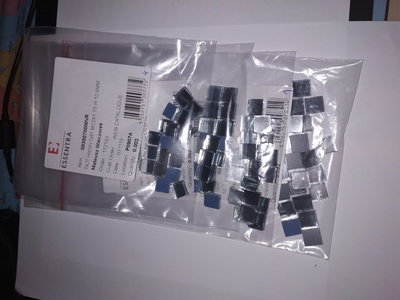
\includegraphics[scale=0.5]{images/1.jpg}
\item Silnik szczotkowy na prąd stały Redox o maksymalnej prędkośći obrotowej 20000 obr./min., poborze prądu przy starcie 7,6 A, podczas pracy 1,8 A, napięciu znamionowym 7,2 V - 1sztuka.

W projekcie został wykorzystany jako napęd wirujących luster odchylających puszczaną na nie wiązkę laserową w kierunku poziomym (potrzebna jest możliwie jak największa prędkość oraz moment obrotowy, dlatego został użyty taki silnik).

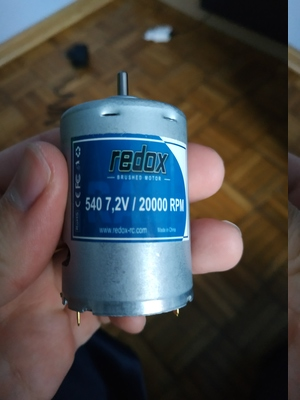
\includegraphics[scale=0.5]{images/2.jpg}
\item Dioda laserowa czerwona 5mW, 650nm, na napięcie 5V, moduł Iduino ST1172 - 1 sztuka.

W projekcie została użyta jako źródło mocnego, skupionego światła, dzięki czemu można było swobodnie manipulować wiązką i nie potrzebne było stosowanie soczewek.
\item Płytka stykowa, 830 otworów, 126 wierszy, 4 magistrale zasilające - 1 sztuka.

W projekcie posłużyła jako płytka prototypowa (podstawa) dla elektroniki projektowane systemu.
\item Mikrokontroler AVR - ATMega8A-PU DIP - 1 sztuka.

W projekcie został użyty jako główny procesor systemu, który za pomocą programatora, taśmy i odpowiednio podpiętych przewodów można było łatwo programować.
\item Programator AVR zgodny z USBasp ISP + taśma IDC - po 1 sztuce.

W projekcie ten zestaw posłużył jako interfejs między komputerem (w którym można było napisać kod źródłowy, na podstawie którego został wygenerowany program dla mikrokontrolera) a mikrokontrolerem (który sterował systemem).
\item Zestaw przewodów połączeniowych 20cm, m-m, m-ż, ż-ż, każdy rodzaj po 40 sztuk.

W projekcie posłużyły jako "luźne" połączenia pomiędzy odpowiednimi komponentami urządzenia. Kilka złączonych razem w jeden przewód stanowiło długi kabel.
\item Zestaw 140 przewodów do płytek stykowych.

W projekcie posłużyły do łączenia wierszy płytki stykowej w celu zbudowania odpowiedniego układu elektronicznego.
\item Zestaw diod LED 5mm - 4 sztuki.

W projekcie posłużyły jako kontrolki - interfejs wyjściowy dla użytkownika.
\item Zestawy rezystorów 1/4W: 10 kOhm, 1 kOhm, 100 Ohm, 1 Ohm.

W projekcie zostały użyte jako rezystory redukujące prąd w poszczególnych obwodach.
\item Nakrętka chromowana do baterii wannowej 3/4 - 1 sztuka.

W projekcie została użyta jako wirujące lustra (gdyż jest to prawdopodobnie symetryczny element, o przekroju poprzecznych zbliżonym do sześciokąta foremnego, posiadający ściane boczne w formie "zwierciadeł płaskich".
\item Odbiornik i nadajnik podczerwieni LiteOn 940nm - 1 para.

W projekcie para tych elementów posłużyła do testowania fazy obrotu nakrętki chromowanej, a przez to i także do zliczania prędkości obrotowej silnika.
\item Tack Switch z nasadką - 5 sztuk.

W projekcie zostały użyte jako przyciski - interfejs wejściowy dla użytkownika.
\item Tranzystor bipolarny NPN BD911 100V/15A - 1 sztuka.

W projekcie został użyty jako "klucz" obwodu silnika pracującego przy wysokim prądzie. Dzięki niemu możliwa była zmiana prędkości obrotowej za pomocą pośrednio podłączonego na bramkę sygnału PWM z mikrokontrolera.
\item Tranzystor bipolarny NPN BC639 80V/1A - 1 sztuka.

W projekcie został wykorzystany w układzie Darlingtona, którego zadaniem było sterowanie obrotami silnika. Był on potrzebny, gdyż szyna zasilająca z portu USB 5V była za słaba aby pełnić tą funkcję prawidłowo.
\item dioda zaporowa o dużym maksymalnym prądzie i napięciu.

W projekcie została wykorzystana jako zabezpieczenie całego układu przed zniszczeniem z powodu odłączenia zasilania z pracującego silnika, który w tej sytuacji pracował jak cewka.
\item Tranzystor unipolarny typu nMOSFET, o małym maksymalnym prądzie i napięciu - 3 sztuki.

W projekcie posłużyły jako elektronika dla mniejszych prądów, bezpośrednio na płytce stykowej.
\item Nakrętka metalowa - 1 sztuka.

W projekcie posłużyła do utrzymywania nakrętki chromowanej oraz możliwie jak najlepszego jej wyśrodkowania.

\item Listewki drewniane, grube tekturki, brzeszczot, klej do drewna.

W projekcie zostały wykorzystane do zbudowania szkieletu konstrukcji, do którego zostały zamontowane poszczególne komponenty.
\end{enumerate}
\subsection{Wydobyte z niedziałających urządzeń przedmioty wykorzystane w projekcie.}
\begin{enumerate}[a)]
\item Wentylator 8cm x 8cm (wydobyty z niesprawnego zasilacza komputerowego)

W projekcie posłużył jako wentylator chłodzący zamontowany radiator, do którego przykręcony był tranzystor sterujący silnikiem (pracując przy wysokim prądzie bardzo szybko się nagrzewał).
\item Prosty radiator - gruba alumiowa płytka (wydobyty z niesprawnego zasilacza komputerowego)

W projekcie posłużył jako radiator tranzystora sterującego pracą silnika.
\item Oraz inne mniejsze rzeczy, które zostały wykorzystane do konstrukcji.

\end{enumerate}
\subsection{Inne wykorzystane urządzenia.}
\item Zasilacz komputerowy.

W projekcie posłużył jako stabilne źródło zasilania elementów nie będących częścią elektroniki cyfrowej.
\begin{enumerate}[a)]
\end{enumerate}
\subsection{Schemat obwodów elektrycznych w ostatecznej wersji urządzenia.}
\begin{figure}[htp] \centering{
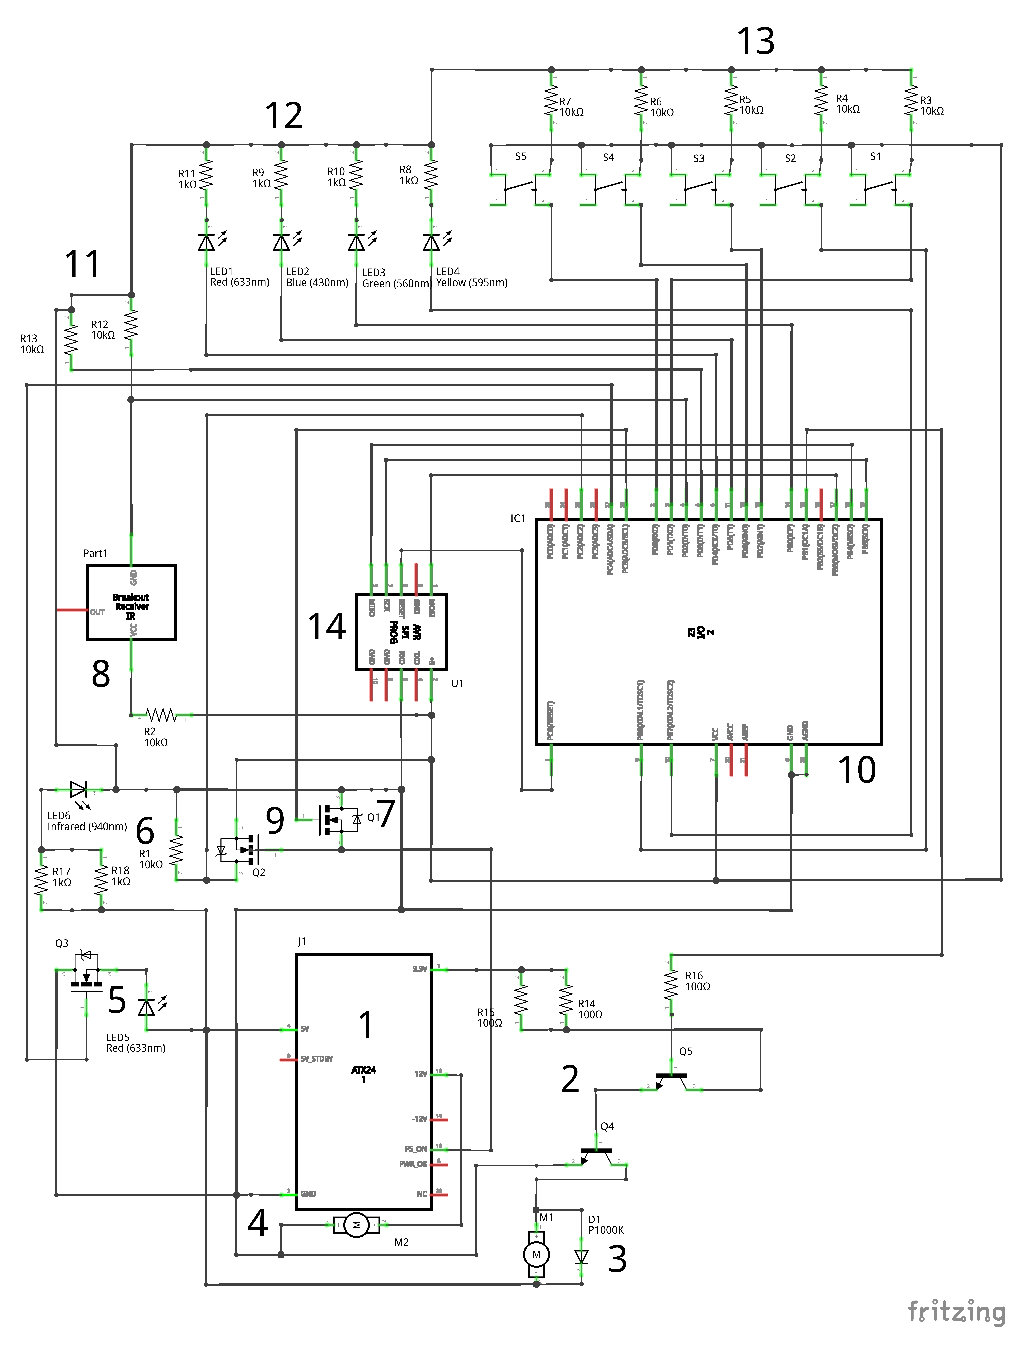
\includegraphics[scale=0.8]{project_schem.pdf}}
\caption{Kompletny schemat obwodów elektrycznych w urządzeniu.}
\end{figure}
\newpage
\subsection{Opis poszczególnych grup zaznaczonych na schemacie.}
\begin{enumerate}[1.]
\item Zasilacz komputerowy.

Zasilacz komputerowy po podłączeniu zasilania jest uruchomiony tylko wtedy, gdy pin PS\_ON jest zwarty z masą tego zasilacza. Takie zwarcie powoduje otwarcie się tranzystora nMOSFET oznaczonego grupą 7. Z tego zasilacza zostały wykorzystane linie 3,3 V, 5V oraz 12V.

\item Układ Darlingtona służący do sterowania pracą silnika wirujących luster.

Na bazę tranzystora NPN Q5 podawany jest sygnał PWM z ATMegi, który w zależności od wypełnienia powoduje szybszą oraz wolniejszą pracę silnika. Przy podawaniu logicznej jedynki tranzystor ten jest otwierany, a obwód 3,3V - rezystory - kolektor i emiter tanzystora Q5 - baza i emiter tranzystora Q4 jest zamykany, w związku z czym tranzystor NPN Q4 (przystosowany do dużych mocy) zaczyna przewodzić prąd. Skutkiem tego jest zamknięcie obwodu 5V - silnik - kolektor i emiter tranzystora Q4, a więc i uruchomienie silnika oznaczonego grupą 3.

Do tego zadania nie można było użyć jedynie tranzystora Q4, gdyż linia 5V z portu USB była zbyt słaba aby otworzyć ten tranzystor (również gwałtownie spadało napięcie w całym obwodzie)

\item Silnik - napęd wirujących luster odchylających wiązkę lasera w poziomym kierunku.

Ten silnik na prąd stały, wysokich obrotów został wykorzystany jak napęd modułu wirujących luster. Ze względu na swoją specyfikację, podczas pracy pobiera duży prąd, a więc i w chwili wyłączania mógłby zniszczyć układ. Z tego powodu została zastosowana dioda zaporowa, która po odłączeniu silnika (który zaczyna pracować jak cewka) zwiera jego piny.

\item Wentylator.

Wentylator dla tego urządzenia zaczął być konieczny po zaimplementowaniu sterowania silnikiem. Tranzystor zamykający obwód silnika, pod wpływem wysokiego prądu zaczął się gwałtownie przegrzewać, przez co było potrzebne przykręcenie go do radiatora. Jednak to nie wystarczało, gdyż wtedy cały radiator zaczął się nagrzewać do wysokich temperatur, zatem trzeba było zapewnić przepływ powietrza wokół radiatora.

\item Obwód lasera - źródła światła w projektorze.

W skład obwodu wchodzi tranzystor nMOSFET małych mocy, który umieszony w obwodzie w kolejności za diodą laserową, działał jak klucz, przez co można było wyłączać i włączać laser. Pomimo napięcia 5V z zasilacza przykładanego na pin anodę diody laserowej, nie potrzebny był tranzystor dużych mocy, gdyż maksymalny pobór prądu wynosił około 25 mA. Na bramkę tranzystora jest podawany sygnał z pinu PC4 mikrokontrolera.

\item Obwód nadajnika podczerwieni.

Jest to prosty obwód z koniecznie dołożonymi rezystorami zmniejszającymi prąd przepływający przez diodę IR. Po uruchomieniu zasilacza nadajnik zaczyna wysyłać promieniowanie podczerwone. Zasilanie z linii 5V zasilacza. Nadajnik wraz z odbiornikiem służą do wyzwalania przerwań układowych w mikrokontrolerze, dzięki czemu urządzenie wie, w której fazie obrotu znajdują się wirujące lustra.

\item Tranzystor służący jako klucz do sterowania pracą zasilacza.

Jest to tranzystor nMOSFET małych mocy, który po otwarciu zwiera pin PS\_ON z pinem masy w zasilaczu, przez co zasilacz się uruchamia. Na bramkę tego tranzystora podawana jest wartość logiczna z pinu PC5 mikrokontrolera.

\item Obwód odbiornika podczerwieni.

Jest to prosty obwód z rezystorem ograniczającym prąd oraz fototranzystorem, który po odebraniu promieniowania podczerwonego się otwiera i zaczyna przewodzić prąd. Obwód zasilany jest linią 5V z portu USB. Po otwarciu tranzystora prąd trafia na pin przerwania układowego 0 mikrokontrolera.

\item Tranzystor służący do testowania obecności zasilania doprowadzanego do zasilacza.

Gdy zasilacza jest włączony przełącznikiem, ale nie pracuje, na pinie PS\_ON pojawia się napięcie 5,5 V. Właśnie to napięcie służy do sprawdzania, czy zasilacz jest gotowy do pracy. Podawane na bramkę tranzystora nMOSFET otwiera go, przez co napięcie 5V z linii z portu USB trafia na pin PC2 mikrokontrolera.

\item Główny mikrokontroler urządzenia - ATMega8A-PU.

Pełni on rolę procesora urządzenia. Jego wykorzystanie i działanie, wraz z kodem źródłowym zostanie przedstawione w dalszych sekcjach.

\item Grupa rezystorów dla pinów przerwań układowych mikrokontrolera.

Zastosowanie tych tranzystorów wymusza przepływ prądu do pinu mikrokontrolera w przypadku logicznej jedynki, natomiast w przypadku logicznego zera = braku prądu łączy z masą.

\item Grupa czterech diod LED - kontrolek. Interfejs wyjściowy dla użytkownika.

Jest to grupa czterech podobnych obwodów elektrycznych. Każdy obwód zaczyna się od określonego pinu (odpowiadającego konkretnej kontrolce), diody LED i rezystora ograniczającego prąd w obwodzie.

\item Grupa pięciu przycisków typu Tact Switch. Interfejs wejściowy dla użytkownika.

Jest to grupa pięciu podobnych do siebie obwodów elektrycznych. W skład każdego obwodu wchodzą: linia 5V z portu USB z jednej strony, masa poprzedzona rezystorem ograniczającym prąd w przypadku naciśnięcia przycisku oraz wyjście do konkretnego pinu mikrokontrolera z drugiej strony. Po naciśnięciu przycisku zwierają sie obie strony, a z powodu obecności rezystora prąd trafia na pin.

\item Programator AVR.

Jest to główny element służący do zasilania elektroniki cyfrowej urządzenia oraz do programowania mikrokontrolera za pomocą linii MISO, MOSI i SCK.
\end{enumerate}
\subsection{Kod źródłowy mikrokontrolera w ostatecznej wersji.}
Kod źródłowy programu mikrokontrolera (wraz z komentarzami) został umieszczony w pliku main.c.
\subsection{Budowanie poszczególnych modułów urządzenia.}
\begin{enumerate}[1.]
\item Moduł wirujących luster.

Był to i jest nadal najtrudniejszy moduł do zaprojektowania i zbudowania. Problemem, który ciągnął się za mną przez cały czas była niemożliwość idealnego osadzenia wirującego komponentu na wale silnika, przez co przy większych obrotach pojawiało się bicie. Pomimo, że wirujący komponent nie wyskakiwał z osi, to powodował on dosyć spore wibracje, które były głośne.
\begin{enumerate}[a)]
\item Na początku był pomysł z zakupieniem lekkiej nakrętki i zwierciadełek płaskich. Po dokonaniu zakupów, przykleiłem zwierciadełka do ścian bocznych nakrętki. Po stestowaniu modułu okazało się, że skończona różna ilość kleju użytego do przyklejnia każdego zwierciadełka powodowała odchylanie wiązki pod różnymi kątami, co było nie do zaakceptowania. Efekt został przedstawiony na filmiku 2.

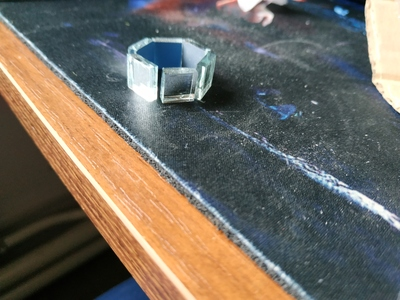
\includegraphics[scale=0.5]{images/3.jpg} 
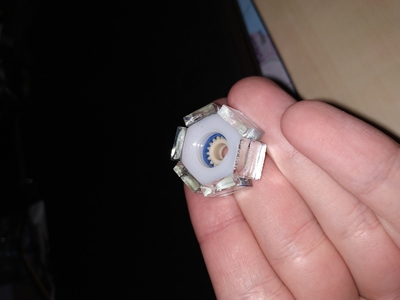
\includegraphics[scale=0.5]{images/4.jpg} 

\item Następnym pomysłem, który ostatecznie zaakceptowałem, było zakupienie nakrętki chromowanej do baterii wannowej, i za pomocą różnych symetrycznych przedmiotów osadzenie jej na wale silnika. Takie rozwiązanie ze względu na to, że proces produkcji takich nakrętek jest bardziej staranny niż ręczne klejenie, umożliwiło odpowiednie osadzenie nakrętki, co pozwoliło na naświetlenie jednej linii za pomocą każdej ze ścian nakrętki. Pomimo owalnych brzegów pomiędzy ścianami bocznymi, część pozostała zwierciadłem płaskim.

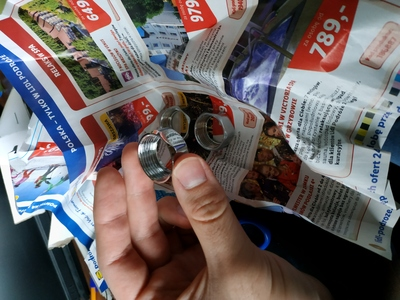
\includegraphics[scale=0.5]{images/5.jpg} 
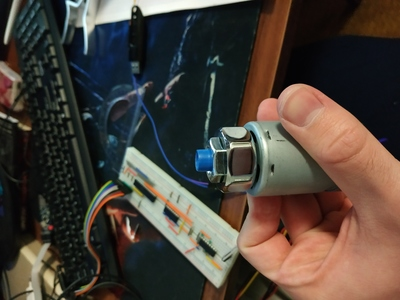
\includegraphics[scale=0.5]{images/6.jpg} 
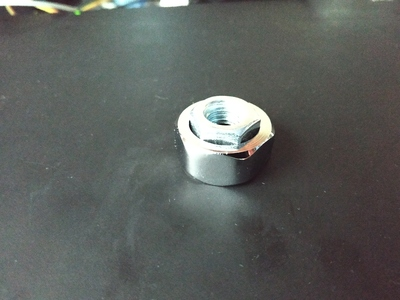
\includegraphics[scale=0.5]{images/7.jpg} 

Jednak z powodu, że ta nakrętka nie była na szytwno osadzona na wale, to wraz prędkością obrotową silnika odchylała się pod minimalnie różnym kątem, co przedstawione zostało na filmiku 1.
\end{enumerate}

\item Moduł napędu wirujących luster.

Był to jeden z większych problemów podczas budowy układu. Z powodu zakupionego silnika wysokich obrotów, pobierał on bardzo duży prąd podczas pracy, a w szczególności podczas startu. Dlatego potrzebne było zastosowanie specjalnego tranzystora przystosowanego na duże prądy. 
\begin{enumerate}[a)]

\item Pierwszym podejściem, po przestraszeniu się działania tranzystorów bipolarnych i ich przewodzenia prądu pomiędzy pinami, zakupiłem tranzystory typu nMOSFET. Jednak z powodu, że pracuje on na wysokich prądach, potrzebował on specjalnego napięcia progowego, aby otworzyć ten tranzystor. Linia 5V z portu USB była tak słaba, że przy obciążeniu przez elektronikę cyfrową oraz inne komponenty, nie wystarczała na jakiekolwiek otwarcie tego tranzystora. Nad tym problemem spędziłem dużo czasu, próbując różnych podejść, czasami również śmiesznych. 

\item Po konsultacjach z prowadzącym okazało się, że ten problem może rozwiązać tranzystor bipolarny, gdyż nie wymaga on odpowiedniego napięcia baza-emiter względem kolektor-emiter. Po zastosowaniu zakupionego na początku tranzystora NPN dużych prądów, problem się znacznie rozwiązał, jednak nadal słaba linia 5V z portu USB nie wystarczała na sterowanie tranzystorem, a w dodatku gwałtownie spadało napięcie na całym obwodzie. Dlatego podświadomie wykorzystałem układ Darlingtona, wykorzystując przy tym tanzystor NPN małych prądów, który było otwierany na podstaiwe sygnału PWM z mikrokontroleta, a to powodowało podanie prądu z linii 3,3 V z zasilacza na bazę właściwego tranzystora. Dzięki temu układowi udało się w 100\% sterować obrotami silnika.

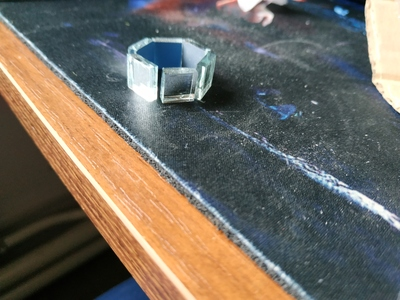
\includegraphics[scale=0.5]{images/3.jpg} 
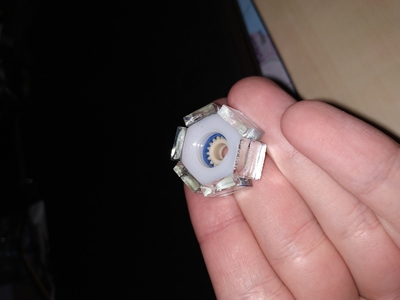
\includegraphics[scale=0.5]{images/4.jpg} 

\end{enumerate}

\item Moduł nadajnika i odbiornika podczerwieni.

Z tym modułem nie było żadnych problemów. Od samego początku spełniał zaplanowane przeze mnie zadanie. Jednak przed wymyśleniem zastosowania takiego układu do sprawdzania fazy obrotu nakrętki minęło dużo czasu. Właściwe podpięcie nadajnika i odbiornika do płyty głównej oraz przede wszystkim właściwe wzajemne ustawienie tych komponentów względem siebie i wirującej nakrętki pozwoliło na bardzo szybki, dokładny i sprawny test fazy obrotu nakrętki (takich faz było 6, gdyż każda ze ścian odbijała w pewnym momencie promieniowanie podczerwone z nadajnika do odbiornika).

Po odebraniu promieniowania podczerwonego, wywoływała się funkcja obsługi przerwania systemowego INT0.

Dzięki odpowiednio napisanej funkcji przedstawionej w sekcji wyżej, udało się uzyskać odpowiednią, zadaną prędkość obrotową silnika. Udokumentowane zostało do na zdjęciach oraz filmiku 4. Dokładna wartość prędkości obrotowej została odczytana przy pomocy przycisków 3 i 4, co również zostało przedstawione na filmiku. Po wciśnięciu przycisku 5, uruchamia się algorytm połówkowego znajdowania PWM, który przy odpowiednim zasilaniu spowoduje, że silnik będzie się obracał z zadaną prędkością. Należy odpowiednio umieścić względem siebie nadajnik i odbiornik podczerwieni, aby lekko świeciła się niebieskia kontrolka. Świeci się ona, gdy wywoływane jest przerwanie układowe. Po jej mignięciu kończy się działanie algorytmu, laży wtedy odstawić moduł, aby zachować ostatnią uzyskaną prędkość obrotową.

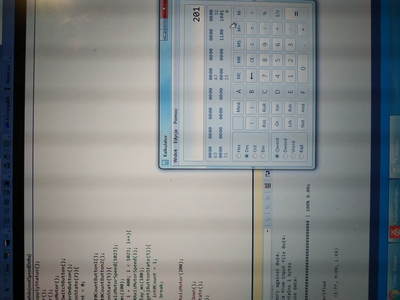
\includegraphics[scale=0.5]{images/8.jpg} 
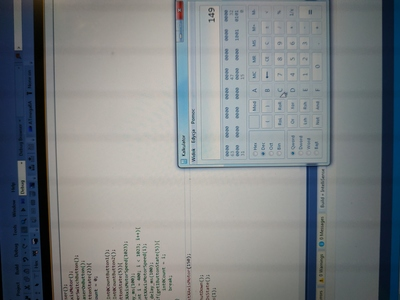
\includegraphics[scale=0.5]{images/9.jpg} 
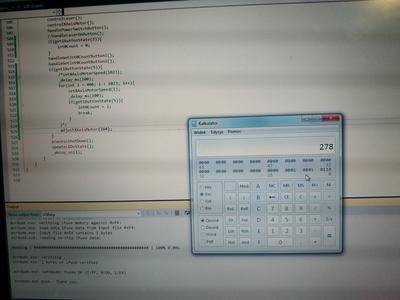
\includegraphics[scale=0.5]{images/10.jpg} 
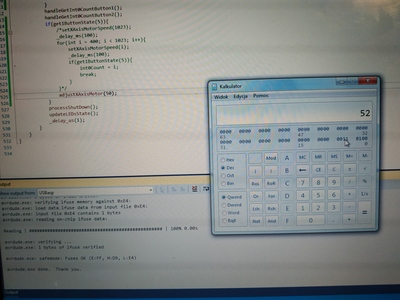
\includegraphics[scale=0.5]{images/11.jpg} 

\item Ogólna konstrukcja urządzenia.

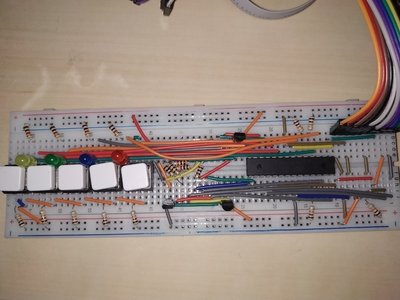
\includegraphics[scale=0.5]{images/12.jpg} 
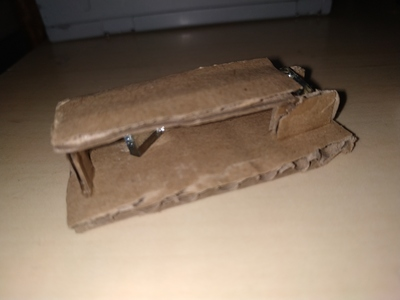
\includegraphics[scale=0.5]{images/13.jpg} 
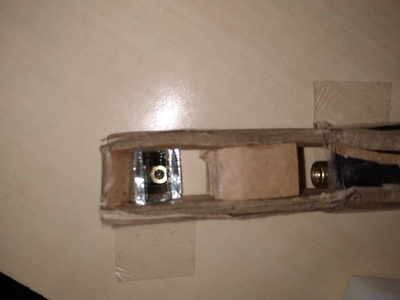
\includegraphics[scale=0.5]{images/14.jpg} 
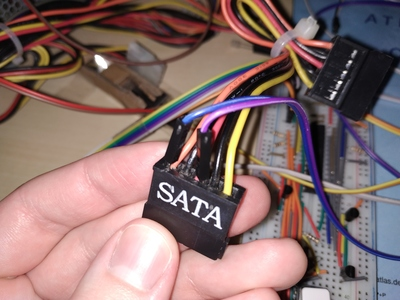
\includegraphics[scale=0.5]{images/15.jpg} 
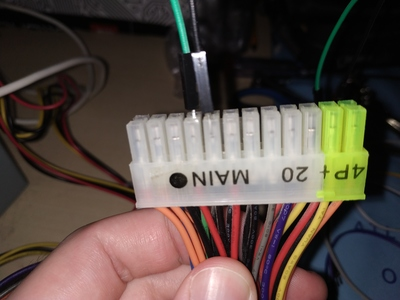
\includegraphics[scale=0.5]{images/16.jpg} 
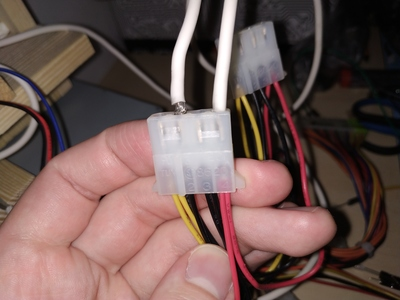
\includegraphics[scale=0.5]{images/17.jpg} 
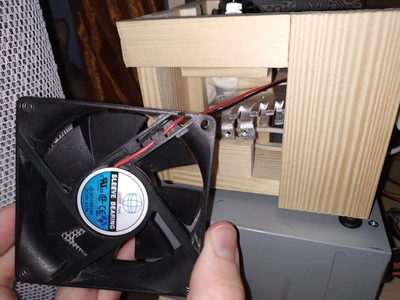
\includegraphics[scale=0.5]{images/18.jpg} 
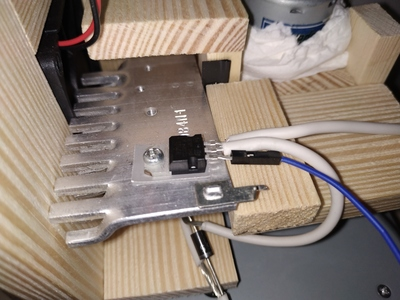
\includegraphics[scale=0.5]{images/19.jpg}
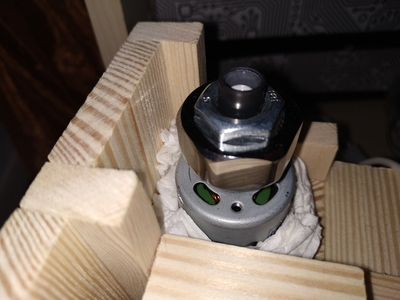
\includegraphics[scale=0.5]{images/20.jpg} 
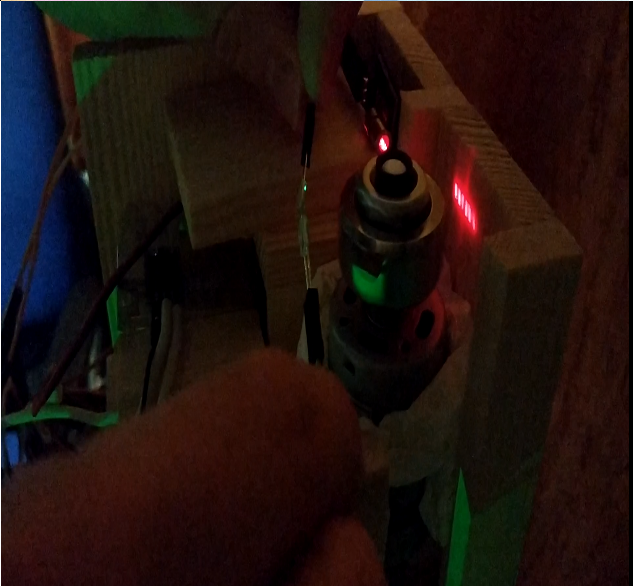
\includegraphics[scale=0.3]{images/21.png} 
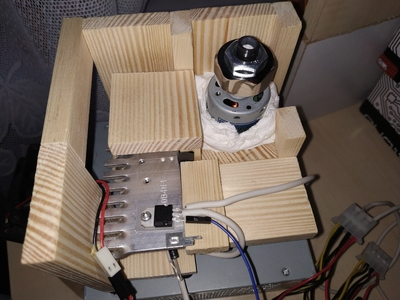
\includegraphics[scale=0.5]{images/22.jpg} 
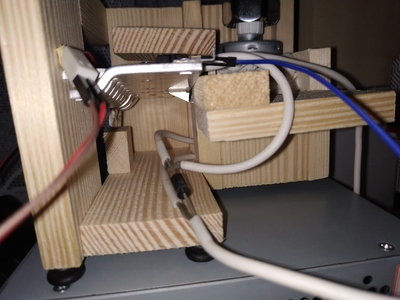
\includegraphics[scale=0.5]{images/23.jpg}
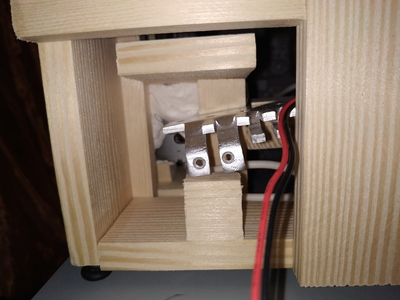
\includegraphics[scale=0.5]{images/24.jpg} 
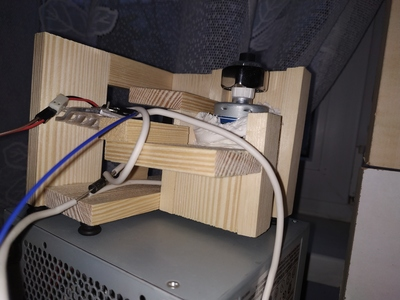
\includegraphics[scale=0.5]{images/25.jpg}
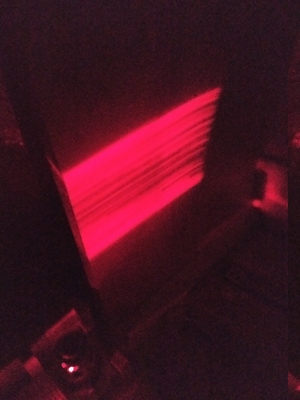
\includegraphics[scale=0.5]{images/26.jpg}
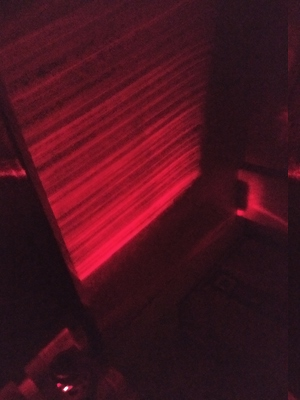
\includegraphics[scale=0.5]{images/27.jpg} 
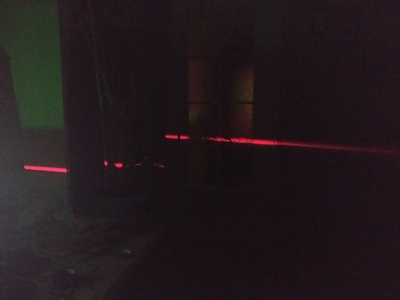
\includegraphics[scale=0.5]{images/28.jpg}



\end{document}